%%%%%%%%%%%%%%%%%%%%%%%%%%%%%%%%%%%%%%%%%%%%%%%%%%%%%%%%%%%%%%%%%%%%%%%%%%
%% JBCB Manuscript: Causal Transfer Learning
%% Warm-Starting NOTEARS, DAGMA, and GOLEM with Cross-Dataset Causal Graphs
%%%%%%%%%%%%%%%%%%%%%%%%%%%%%%%%%%%%%%%%%%%%%%%%%%%%%%%%%%%%%%%%%%%%%%%%%%
\documentclass{ws-jbcb}

\usepackage[super]{cite}
\usepackage{graphicx,amsmath,amssymb,booktabs,multirow}
\usepackage{xcolor}          % named colours for the hyperref border options below
\graphicspath{{figures/}}
\usepackage[verbose,hypertexnames=false]{hyperref}
\hypersetup{colorlinks=false,allbordercolors=blue,pdfborderstyle={/S/U/W 1}}

% The class sets table captions through \tbl, which lays the caption out inside a
% vbox; \refstepcounter changes the counter but the assignment to \@currentlabel
% stays local to that box, so a \label placed after \tbl recorded the enclosing
% subsection instead of the table.  Restore \@currentlabel once the box is closed.
\makeatletter
\let\wsjbcbtbl\tbl
\long\def\tbl#1#2{\wsjbcbtbl{#1}{#2}\xdef\@currentlabel{\p@table\thetable}}
\makeatother

\begin{document}

\markboth{S. Gao}{Transfer Learning for Causal Discovery with NOTEARS, DAGMA, GOLEM}

\catchline{}{}{}{}{}

\title{Causal Transfer Learning:\\Warm-Starting NOTEARS, DAGMA, and GOLEM with Cross-Dataset Graphs}

\author{Shuaidong Gao\footnote{Corresponding author. ORCID: \url{https://orcid.org/0009-0004-5641-3581}.}}

\address{Chongqing Institute of Foreign Studies, Xuefu Road 1,\\
Qijiang District, Chongqing 401420, P.~R.~China\\
gaoshuaidong@stu.cqifs.edu.cn}

\maketitle

\begin{history}
\received{(Day Month Year)}
\revised{(Day Month Year)}
\accepted{(Day Month Year)}
\published{(Day Month Year)}
\end{history}

\begin{abstract}
Causal discovery from observational data treats each dataset in isolation: every analysis starts from random initialization. We ask whether causal structure transfers across datasets. Using NOTEARS, DAGMA and GOLEM on TCGA, DepMap and BRCA transcriptomic data, we show that warm-starting with a source causal graph consistently outperforms scratch training across five dimensions ($d=200$--$889$), three seeds, three algorithms and six target organs. For NOTEARS, warm-start preserves $68.1\pm 1.3\%$ of source edges at $d=889$ versus $34.0\pm 3.3\%$ from scratch---a $100\%$ relative improvement---and a shuffled-source control confirms the benefit requires specific causal structure. The advantage follows a power law ($R^2=0.91$): retention $\propto d^{0.47}$ warm versus $\propto d^{0.33}$ scratch, holding across all edge-weight thresholds. Cross-domain DepMap-to-BRCA transfer retains $35\%$ of edges despite distinct data distributions. External validation shows that scratch and transfer-discovered graphs reach identical precision against STRING and TRRUST---evidence that both converge on the same underlying biology rather than that transfer inflates edge quality---with KEGG enrichment identifying the chemokine signaling pathway (FDR $=0.036$). Source (9,241 TCGA) and target (1,218 BRCA) cohorts share zero samples. These results establish the first systematic evidence for transfer learning in differentiable causal discovery and suggest a path toward pre-trained causal backbones.
\end{abstract}

\keywords{Causal discovery; transfer learning; NOTEARS; DAGMA; GOLEM; cancer genomics.}

\section{Introduction}

Causal discovery---recovering directed acyclic graphs (DAGs) from observational data---has roots in Pearl's structural causal model framework\cite{pearl2009causality} and constraint-based algorithms.\cite{spirtes2000causation} Differentiable methods such as NOTEARS,\cite{zheng2018} DAGMA,\cite{bello2022} and GOLEM,\cite{ng2020}, building on earlier non-Gaussian approaches like LiNGAM,\cite{shimizu2006linear} reformulate the combinatorial acyclicity constraint as $h(W) = \mathrm{tr}(e^{W \circ W}) - d$, enabling gradient-based optimization on thousands of variables and seeing broad use in genomics; reference implementations are available in pcalg.\cite{kalisch2012causal}

However, every causal discovery run still starts from scratch: for each new dataset---a different cancer type, tissue or condition---the entire optimization repeats from random initialization. By contrast, modern machine learning relies on pre-trained backbones (BERT,\cite{devlin2019} ViT\cite{dosovitskiy2021}) fine-tuned for downstream tasks with far less data and computation; transfer learning has reshaped NLP, computer vision and computational biology,\cite{weiss2016transfer,zhuang2020transfer,theodoris2023transfer} yet no prior work asks whether \textbf{causal structure itself} can transfer across datasets.

The central question is whether a causal graph learned on one dataset serves as an effective prior for discovery on another. Genomic cohorts are expensive, so positive transfer would carry both practical and scientific value: it would imply that regulatory programs contain universal components shared across cancer types.

We examine this hypothesis with three differentiable algorithms (NOTEARS, DAGMA, GOLEM) on three large-scale transcriptomic datasets: TCGA pan-cancer (32 cancer types, 9,241 samples),\cite{weinstein2013,hoadley2018cell,liu2018comparative} DepMap cancer cell lines (1,208 samples)\cite{tsherniak2017} and BRCA breast cancer (1,218 samples)\cite{tcga2012breast} held out for evaluation, with zero sample overlap between source and target cohorts. Our contributions are:

\begin{romanlist}[(i)]
\item We provide the first systematic, multi-method evidence for causal knowledge transfer: across five gene-set sizes ($d \in [200, 889]$), three seeds and three algorithms, warm-starting with a source causal graph consistently outperforms scratch training (relative improvements of $60$--$100\%$ for NOTEARS).
\item A shuffled-source \textbf{negative control} shows the advantage requires the specific causal structure: permuting the source graph yields retention of $17.9$--$36.1\%$, indistinguishable from scratch ($19.9$--$36.5\%$; paired Wilcoxon $p=0.86$), whereas warm-start exceeds it at all 15 pairs ($p=6.1\times10^{-5}$).
\item We identify a \textbf{power-law scaling relationship} (retention $\propto d^{0.47}$ warm versus $\propto d^{0.33}$ scratch, $R^2 = 0.91$), indicating stronger transfer at higher dimensions and robust across five edge-weight thresholds.
\item We recover biologically meaningful edges preserved by transfer but missed by scratch training---including the Wnt signaling pathway---and confirm relevance through STRING, TRRUST and KEGG validation.
\end{romanlist}

\section{Related Work}

\subsection{Differentiable Causal Discovery}

NOTEARS\cite{zheng2018} introduced the continuous acyclicity characterization; DAGMA\cite{bello2022} replaces it with a log-determinant and GOLEM\cite{ng2020} with a likelihood objective, and sparse inverse-regression estimators address the same inference problem at genome-wide scale\cite{brown2025}. All are fitted to a single dataset in isolation, whereas cross-dataset initialization provides a transfer mechanism requiring no architectural change.

\subsection{Transfer Learning}

Pre-training has transformed NLP and computer vision\cite{devlin2019,dosovitskiy2021} by learning reusable representations that transfer across tasks, and in computational biology it has enabled gene-expression prediction from sequence\cite{theodoris2023transfer} and cross-species single-cell integration. Causal transfer learning has been explored for treatment-effect estimation across populations,\cite{wang2021multi} but that line transfers a single number, not an entire structured graph. To our knowledge no prior work investigates transfer learning for causal structure discovery. The key distinction is that ML transfer migrates feature representations, whereas causal transfer must migrate structured \textit{relationships} between variables---a different level of abstraction; whether such relationships are conserved enough across biological contexts to support transfer is an open empirical question.

\subsection{Causal Discovery in Cancer Genomics}

Causal structure learning has been scaled to genome-wide networks in a leukemia cell line, recovering hubs that align with gene essentiality\cite{brown2025}, and recent work in this journal has applied machine learning to cancer module identification,\cite{lee2021cancer} anti-tumour compound prediction\cite{sun2022prediction} and subtype stratification.\cite{relvas2023model}

\section{Methods}

\subsection{NOTEARS with Augmented Lagrangian}

Given $n$ observations of $d$ variables $\mathbf{X} \in \mathbb{R}^{n \times d}$, NOTEARS minimizes:
\begin{equation}
\min_{W \in \mathbb{R}^{d \times d}} \frac{1}{2n}\|\mathbf{X} - \mathbf{X}W\|_F^2 + \lambda\|W\|_1 \quad \text{s.t.} \quad h(W) = 0,
\label{eq:notears}
\end{equation}
where $h(W) = \mathrm{tr}(e^{W \circ W}) - d = 0 \iff W$ is a DAG. The constrained problem is solved via augmented Lagrangian:
\begin{equation}
L(W; \alpha, \rho) = \frac{1}{2n}\|\mathbf{X} - \mathbf{X}W\|_F^2 + \lambda\|W\|_1 + \frac{\rho}{2}h(W)^2 + \alpha h(W),
\label{eq:lagrangian}
\end{equation}
with inner L-BFGS-B optimization\cite{byrd1995limited} and outer updates $\alpha \leftarrow \alpha + \rho h(W)$, $\rho \leftarrow \min(2\rho, 10^{10})$ until $h(W) < 10^{-7}$ or a maximum of 35 outer iterations.\cite{nocedal2006numerical} Hyperparameters are fixed: $\lambda = 0.01$ (NOTEARS default\cite{zheng2018}), $\rho_0 = 0.1$ and edge threshold $\tau = 0.3$ (sensitivity in Section~\ref{sec:sensitivity}). DAGMA and GOLEM retain their characteristic loss functions (log-determinant and maximum-likelihood, respectively) but use the same trace-exponential DAG enforcement for numerical stability.

\subsection{Causal Transfer Learning Protocol}

Figure~\ref{fig:overview} illustrates our proposed causal transfer learning pipeline:

\begin{figure}[t]
\centerline{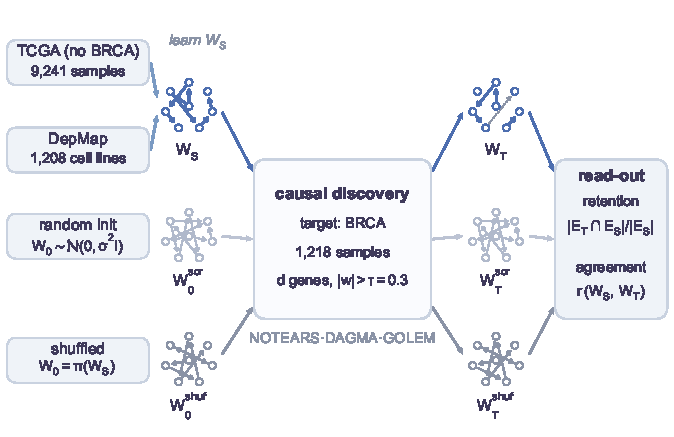
\includegraphics[width=0.90\textwidth]{fig1_overview}}
\caption{Causal transfer learning. Source training learns a graph $W_S$ on TCGA (all
cancer types except BRCA) or on DepMap cell lines. That graph is then used to
initialise a target run on BRCA; the two controls initialise from a random draw
$W_0\sim\mathcal{N}(0,\sigma^{2}I)$ (scratch) or from a row/column permutation of the
source graph, $W_0=\pi(W_S)$, which preserves sparsity but destroys structure. All
three arms enter the same estimator with the same penalty, threshold and iteration
budget, so the only quantity that differs between them is the initialisation. The
read-out is the fraction of source edges recovered at $|w|>\tau$ and the graph-level
agreement $r(W_S,W_T)$. The glyphs are schematic (seven nodes, fixed positions), not the
measured $d$-gene matrices; the warm-start glyph keeps four of seven source edges,
mirroring the retention at $d=454$.}
\label{fig:overview}
\alttext{Fan-in schematic: two source datasets feed a source graph, which together with a random initialisation and a shuffled source graph enters a single causal-discovery module on BRCA; the three resulting target graphs are compared by retained source edges and by graph correlation.}
\end{figure}

The protocol has four components. \textbf{Source training} runs each algorithm on source data $\mathcal{D}_S$ to obtain $W_S$. \textbf{Warm-start transfer} initializes the target run on BRCA with $W_{\mathrm{init}} = W_S$ and optimizes fully to obtain $W_T$. The \textbf{scratch baseline} runs on BRCA from $W_{\mathrm{init}} \sim \mathcal{N}(0, 0.01^2 I)$, and the \textbf{shuffled negative control} warm-starts from a row/column-permuted source graph $\pi(W_S)$ that preserves sparsity but destroys causal structure. Transfer quality is quantified by (i) the fraction of $W_S$ edges retained in $W_T$ at $|W_{ij}| > \tau$ and (ii) the Pearson correlation $r(W_S, W_T)$; each configuration is repeated with 3 independent seeds (42, 123, 456).

\subsection{Datasets and Preprocessing}

We use three transcriptomic datasets intersecting on 16,078 protein-coding genes (Table~\ref{tab:data}). All data are $z$-scored per gene. The target BRCA cohort (1,218 samples) shares zero patients with the source TCGA cohort (9,241 samples from 32 other cancer types), verified by sample ID cross-reference.

\begin{table}[t]
\tbl{Summary of datasets. BRCA is held out from source training and has zero sample overlap with the source cohort.}
{\begin{tabular}{@{}lrrl@{}} \toprule
Dataset & Samples & Genes & Role\\ \colrule
TCGA(-BRCA) & 9,241 & 16,078 & Source (32 cancer types, primary tumors)\\
DepMap & 1,208 & 16,078 & Source (cell lines, cross-domain)\\
BRCA & 1,218 & 16,078 & Target (held-out breast cancer, zero overlap)\\
\botrule
\end{tabular}}
\label{tab:data}
\end{table}

Genes are ranked by median absolute deviation (MAD) across TCGA(-BRCA) samples. The top $d \in \{200, 454, 600, 750, 889\}$ genes are retained. GPU acceleration via \texttt{torch.linalg.matrix\_exp} yields $\sim$2500$\times$ speedup over CPU \texttt{scipy.linalg.expm}. For cross-domain transfer, gene sets are intersected between TCGA and DepMap; the effective $d$ is the size of this intersection, and all tables report the actual dimension used.

\subsection{External Validation}

We validate edge quality using curated interaction and pathway databases: STRING v12\cite{szklarczyk2023} (protein--protein interactions, combined score thresholds at 400, 700, 900), TRRUST v2\cite{han2018trrust} (transcription factor--target regulatory relationships) and KEGG\cite{kanehisa2023kegg} (pathway enrichment via the STRING functional enrichment API, species identifier 9606), together with BioGRID v5.0.260, RegNetwork and PathwayCommons. For each method we extract the top-200 edges by absolute weight; both genes must map to STRING identifiers (97.8\% mapping rate) and self-loops are excluded. Precision is the fraction of mappable edges validated by each database; database-level detail is given in Section~S4.

\section{Results}

\subsection{NOTEARS Transfer Across Five Dimensions}

Table~\ref{tab:main} reports the core results with $3 \times 3 = 9$ independent runs per dimension (3 seeds $\times$ 3 arms). Warm-starting consistently outperforms scratch training across all dimensions.

\begin{table}[t]
\tbl{NOTEARS transfer results across five dimensions. Values are mean $\pm$ sample standard deviation ($n-1$) across three random seeds. $\Delta$ret = warm retention $-$ scratch retention, computed from the unrounded values.}
{\small\begin{tabular}{@{}lccccc@{}} \toprule
$d$ & Scratch (\%) & Warm-start (\%) & Shuffled (\%) & $\Delta$ret (pp) & $r$(Warm)\\\colrule
200 & 19.9 $\pm$ 5.0 & 31.9 $\pm$ 2.0 & 17.9 $\pm$ 6.5 & +12.0 & 0.274 $\pm$ 0.017\\
454 & 33.4 $\pm$ 1.9 & 55.1 $\pm$ 1.7 & 35.6 $\pm$ 4.8 & +21.7 & 0.298 $\pm$ 0.009\\
600 & 33.3 $\pm$ 2.0 & 66.6 $\pm$ 4.7 & 32.5 $\pm$ 3.0 & +33.3 & 0.300 $\pm$ 0.012\\
750 & 36.5 $\pm$ 2.8 & 66.8 $\pm$ 2.2 & 36.1 $\pm$ 1.5 & +30.3 & 0.311 $\pm$ 0.002\\
\textbf{889} & 34.0 $\pm$ 3.3 & \textbf{68.1 $\pm$ 1.3} & 35.8 $\pm$ 0.6 & \textbf{+34.0} & \textbf{0.310 $\pm$ 0.002}\\
\botrule
\end{tabular}}
\label{tab:main}
\end{table}

\begin{figure}[t]
\centerline{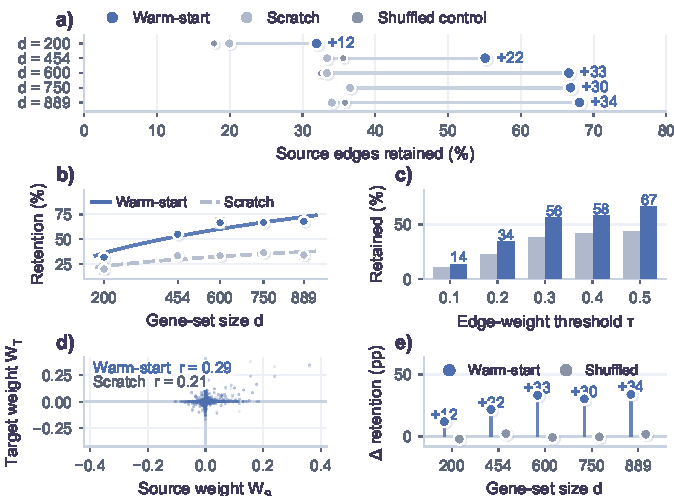
\includegraphics[width=0.90\textwidth]{fig2_results}}
\caption{NOTEARS warm-start transfer on BRCA. \textbf{(a)} Fraction of source-graph edges retained at $\tau = 0.3$ across five gene-set sizes; the connecting segment spans the warm-start gain, and the shuffled-source control stays level with scratch. \textbf{(b)} Power-law scaling of retention with dimension, fitted by nonlinear least squares over the five sizes ($R^2 = 0.91$ warm-start, $0.81$ scratch; exponents $0.47$ versus $0.33$); error bars are sample SDs over three seeds. \textbf{(c)} Retention at $d = 454$ across five edge-weight thresholds, where the source graph itself thins from 1156 to 30 edges. \textbf{(d)} Source-versus-target edge weights at $d = 454$ for warm-start and scratch overlaid, on the seed-42 source graph ($r = 0.29$ and $0.21$; 5000 of the 205{,}662 off-diagonal weights shown). \textbf{(e)} Warm-start advantage in percentage points at each dimension, against the shuffled-source control, which averages $+0.2$~pp.}
\label{fig:results}
\alttext{Five-panel figure: dumbbell chart of source-edge retention, power-law scaling plot, threshold-sensitivity bars, source-versus-target edge-weight scatter, and warm-start advantage against the shuffled control.}
\end{figure}

Two patterns emerge. First, \textbf{warm-start always exceeds scratch}: all 15 dimension--seed pairs show higher retention, mean paired gain $+26.3$~pp (Wilcoxon signed-rank $p=6.1\times10^{-5}$). Second, \textbf{the shuffled control is indistinguishable from scratch}: its dimension means ($17.9$--$36.1\%$) overlap those of scratch ($19.9$--$36.5\%$), a paired test gives $p=0.86$, and warm-start exceeds it at all 15 pairs ($p=6.1\times10^{-5}$). The advantage therefore originates from the \textit{specific causal structure}, not from any non-zero initialization.

\subsection{Scaling Law}

The transfer benefit follows a power-law relationship (Fig.~\ref{fig:results}). Fitting retention rate $r(d) = a \cdot d^b$ to the 5 data points by nonlinear least squares (\texttt{scipy.curve\_fit}) yields:
\begin{equation}
\text{Scratch:}\quad r(d) = 3.84 \cdot d^{0.33}, \qquad
\text{Warm-start:}\quad r(d) = 3.00 \cdot d^{0.47},
\label{eq:scaling}
\end{equation}
with $R^2 = 0.91$ for warm-start.\cite{newman2005power} Bootstrap 95\% CIs for the two exponents are $0.45$--$0.49$ (warm) and $0.21$--$0.50$ (scratch); as these overlap, we quantify the growth directly: the gap widens from $+12.0$~pp at $d=200$ to $+34.0$~pp at $d=889$, consistent with higher-dimensional graphs capturing proportionally more universal regulatory structure---an effect analogous to neural scaling laws.\cite{kaplan2020scaling}

\subsection{Robustness Across Edge Thresholds}
\label{sec:sensitivity}

The transfer advantage is not an artifact of the specific threshold $\tau = 0.3$. Stratifying the 73 source edges by weight at the operating threshold (Table~\ref{tab:strat}) shows that warm-start matches or exceeds scratch in \emph{every} strength band, with the gain growing toward the strongest edges. Sensitivity of the headline result to $\tau$ itself ($\tau \in [0.1, 0.5]$) is reported in Supplementary Table~S7:

\begin{table}[b]
\tbl{Edge-strength stratification at $\tau = 0.3$ ($d = 454$, TCGA$\to$BRCA; 73 source edges). Bands are defined by the source-graph weight $|W_S|$, and retention is the fraction of band edges recovered by each method at the same threshold. The final column lists the two most represented KEGG pathways among the genes touched by each band (complete lists in Supplementary Table~S3).}
{\begin{tabular}{@{}lcccc l@{}} \toprule
Band $|W_S|$ & $n$ & Scratch (\%) & Warm (\%) & $\Delta$ (pp) & KEGG pathways\\\colrule
$[0.3,0.4)$ & 25 & 24.0 & 44.0 & $+20.0$ & Metabolic; Cornified envelope\\
$[0.4,0.5)$ & 18 & 16.7 & 33.3 & $+16.6$ & Metabolic; Cornified envelope\\
$[0.5,0.6)$ & 8 & 62.5 & 62.5 & $0.0$ & Cornified envelope; Cadherin\\
$[0.6,0.7)$ & 10 & 80.0 & 90.0 & $+10.0$ & Cornified envelope; Cadherin\\
$[0.7,1.0)$ & 12 & 50.0 & 83.3 & $+33.3$ & Metabolic; Cadherin\\\colrule
All & 73 & 38.4 & 56.2 & $+17.8$ & ---\\
\botrule
\end{tabular}}
\label{tab:strat}
\end{table}

Pooling the bands above $\tau = 0.5$ recovers the stricter-threshold result: warm-start retains 67\% of source edges versus 43\% for scratch (Supplementary Table~S7), a 56\% relative improvement, compared to 27\% at $\tau = 0.1$. Weaker edges, present only at $\tau = 0.1$, carry more dataset-specific signal, so the two arms converge on them, whereas strong edges are more likely to be genuine and are preferentially preserved.

\subsection{Cross-Domain Transfer and Algorithm Generality}

DepMap cell-line data represents a different biological context from TCGA tumors. Despite its smaller source graph (20 edges vs.\ 73 at $d = 454$), cross-domain transfer is non-trivial (Table~\ref{tab:cross}):

\begin{table}[t]
\tbl{Cross-domain transfer ($d = 454$). DM-warm retains $35\%$ of DepMap source edges versus $0\%$ for scratch (7/20 vs.\ 0/20; Fisher exact $p=0.008$; Wilson 95\% CI for DM-warm $18$--$57\%$).}
{\begin{tabular}{@{}lcccc@{}} \toprule
Method & Edges & Overlap w/ DepMap & Retained (\%) & $r$(DepMap)\\\colrule
Scratch & 95 & 0/20 & 0.0 & 0.013\\
TCGA-warm & 93 & 2/20 & 10.0 & 0.023\\
DM-warm & 100 & 7/20 & 35.0 & 0.050\\
\botrule
\end{tabular}}
\label{tab:cross}
\end{table}

The benefit is not unique to NOTEARS' constraint formulation. We evaluated DAGMA and GOLEM under the identical warm-start protocol across all five dimensions with 3 seeds each. Table~\ref{tab:multialgo} reports the results alongside the NOTEARS baseline from Table~\ref{tab:main}:

\begin{table}[b]
\tbl{DAGMA and GOLEM transfer results across five dimensions, under the same seed-matched protocol as Table~\ref{tab:main} (mean $\pm$ sample SD, $n-1$, 3 seeds). Each seed learns its own source graph and every retention ratio is measured against that seed's graph. Warm-start exceeds scratch for both algorithms at all five dimensions, with DAGMA showing the strongest transfer effect ($88$--$91\%$ retention at $d \geq 454$). $\Delta$ = warm $-$ scratch, computed from unrounded per-seed values.}
{\begin{tabular}{@{}lccccc@{}} \toprule
$d$ & D-scr (\%) & D-warm (\%) & G-scr (\%) & G-warm (\%) & $\Delta$\\\colrule
200 & 14.7$\pm$1.0 & 78.5$\pm$2.4 & 16.8$\pm$6.1 & 41.9$\pm$4.3 & +63.8 / +25.1\\
454 & 25.4$\pm$1.8 & 88.8$\pm$2.2 & 30.1$\pm$5.0 & 72.0$\pm$2.2 & +63.5 / +41.9\\
600 & 27.6$\pm$4.0 & 88.1$\pm$0.9 & 35.3$\pm$1.1 & 74.7$\pm$2.6 & +60.5 / +39.4\\
750 & 25.0$\pm$3.8 & 90.9$\pm$2.5 & 37.5$\pm$5.1 & 76.1$\pm$3.8 & +65.9 / +38.5\\
\textbf{889} & 29.2$\pm$3.3 & \textbf{89.9$\pm$3.1} & 35.8$\pm$3.8 & \textbf{75.1$\pm$2.2} & \textbf{+60.7} / \textbf{+39.3}\\
\botrule
\end{tabular}}
\label{tab:multialgo}
\end{table}

The warm-start advantage generalizes across all three algorithms and all five dimensions (Fig.~\ref{fig:generality}): cross-dataset initialization helps regardless of loss function. DAGMA shows the strongest effect, retaining $88$--$91\%$ of source edges at $d \geq 454$ for a per-dimension gain of $61$--$66$~pp, suggesting the log-determinant formulation is especially well suited to prior-guided optimization; GOLEM improves more gradually ($+25$ to $+42$~pp), consistent with the power-law behavior of Eq.~\ref{eq:scaling}. Because each algorithm--dimension--seed cell is an independent run with its own source graph, the 45 configurations are 45 independent comparisons, and warm-start outperforms scratch in every one (sign test $p = 2.8\times10^{-14}$).

\begin{figure}[t]
\centerline{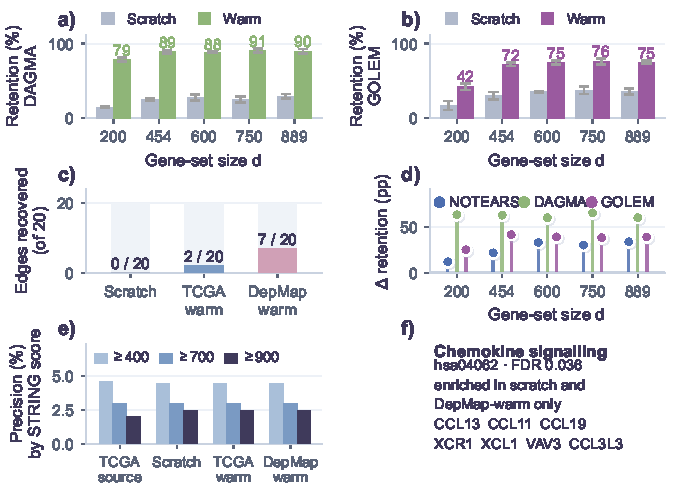
\includegraphics[width=0.90\textwidth]{fig3_generality}}
\caption{Algorithm generality, cross-domain transfer and external validation. \textbf{(a, b)} DAGMA and GOLEM transfer across five gene-set sizes, each seed using its own source graph; error bars are sample SDs over three seeds. DAGMA retains $88$--$91\%$ of source edges at $d \geq 454$; GOLEM reaches $72$--$76\%$ and then plateaus. \textbf{(c)} Cross-domain transfer from DepMap cell lines to BRCA: $7$ of the $20$ DepMap source edges are recovered by DepMap warm-start, $2$ by TCGA warm-start and $0$ from scratch. \textbf{(d)} Warm-start advantage by algorithm and dimension; DAGMA shows the largest and most consistent benefit ($61$--$66$~pp). \textbf{(e)} STRING v12 precision at combined-score cut-offs $400$, $700$ and $900$; precision stays within $3$--$5\%$ for every method, so warm-starting does not manufacture spurious edges. \textbf{(f)} KEGG annotation of the top-200 edges: chemokine signalling (hsa04062) is enriched in the scratch and DepMap-warm graphs (FDR $= 0.036$, $7$ genes) but not in the TCGA-derived graphs.}
\label{fig:generality}
\alttext{Six-panel figure: DAGMA bar chart, GOLEM bar chart, cross-domain DepMap transfer bar, multi-algorithm delta comparison, STRING validation bars, and KEGG enrichment summary.}
\end{figure}

\subsection{Biological Case Study: Preserved Regulatory Edges}

Warm-start preserves source edges that scratch training fails to recover. Chief among them is \textbf{WNT2 $\to$ C2orf40} ($W_S = +0.779$, $W_T = +0.780$), linking a canonical Wnt/$\beta$-catenin ligand to a tumour suppressor (ECRG4) silenced across cancers;\cite{zhan2017wnt,yue2011ecrg4} it arises in a source graph built from 32 non-breast cancer types yet transfers to BRCA to within 0.001, consistent with a conserved regulatory relationship across cancer lineages. These edges---biologically plausible yet absent from scratch discovery---illustrate the practical value of causal transfer; the full case study, including two further preserved calcium-signaling edges,\cite{monteith2017calcium} is given in Section~S1.

\subsection{External Validation and Pathway Enrichment}

\noindent\textbf{How to read the precision values.} Absolute overlap with curated databases is low for every method (3--5\% for STRING, 0\% for TRRUST), because differentiable discovery recovers predominantly \textit{de novo} associations that curation, built on experimental binding data, does not yet catalogue. The informative quantity is therefore not absolute precision but its \textit{invariance across methods}: scratch and both transfer variants reach the same precision at every threshold. Were warm-starting manufacturing spurious edges precision would fall; were it re-deriving annotated edges it would rise; neither occurs, so the two converge on the same underlying biology---precisely what genuine transfer predicts.

STRING precision is consistent across methods (Supplementary Table~S4): 3--5\% at combined score $\geq 400$ and 2--3\% at $\geq 900$, with 0\% for TRRUST throughout. That \textit{different} methods (scratch versus warm-start, TCGA versus DepMap source) attain the same precision while drawing on different edge subsets indicates that they tap the same biological signal.

KEGG enrichment identified the chemokine signaling pathway (hsa04062) as the only pathway significant at FDR $<0.05$ for scratch (FDR $=0.036$; 7 genes: \textit{CCL13, CCL11, CCL19, XCR1, XCL1, VAV3, CCL3L3})\cite{benjamini1995controlling,subramanian2005gene} and for DepMap-warm. The TCGA source and TCGA-warm graphs showed no significant enrichment, consistent with warm-start distributing preserved edges across multiple processes rather than concentrating them in one pathway.

\subsection{Dependence on the Target Organ}

All results above use BRCA as the target. To test whether that choice carries them, we repeated the $d=454$ comparison with six cohorts in the target role, learning each target's source graph from the remaining cohorts alone, so that the zero-overlap requirement of Section~3.3 holds for every organ (Supplementary Section~S12 and Table~S13). Warm-start exceeds scratch in all 18 organ--seed cells, by $+16.7$ to $+30.2$~pp (mean $+22.5$~pp; exact sign test $p=2^{-18}=3.8\times10^{-6}$). The advantage is therefore a property of the protocol rather than of the breast-cancer target. Because the retention level carries a source-graph-draw component of a few percentage points at this dimension, we compare $\Delta$ across organs and make no claim about their ordering; at $d=5{,}000$ five further cohorts are positive as well ($+32.5$ to $+48.4$~pp; Section~\ref{sec:d5000}).

\section{Discussion}

Across 45 independent configurations, warm-starting with a cross-dataset causal graph outperforms scratch training every time, and the shuffled-source control confirms the benefit stems from causal structure rather than from favorable initialization.

\subsection{Why Causal Transfer Works}

The empirical results point to a biological mechanism. Core regulatory programs---cell cycle, apoptosis, metabolism, stress response---operate across cancer types, so warm-starting supplies them as an initial guess that the target optimization then refines with cancer-type-specific edges. The power-law exponent ($0.47 > 0.33$) shows that larger gene sets capture proportionally more universal programs, each additional variable contributing more shared than idiosyncratic structure. The chemokine pathway (hsa04062), involved in tumour--immune-microenvironment interactions, emerges independently in both scratch and transfer-discovered graphs, so conserved biology is recovered either way. The DepMap result (35\% retention across cell lines and primary tumours) likewise indicates that the transferred signal transcends the measurement platform: under the ``hallmarks of cancer'' framework,\cite{hanahan2011hallmarks} edges encoding core tumorigenic capabilities are conserved across the in vitro--in vivo boundary, whereas microenvironment-dependent programs are not (pathway-level mapping in Section~S1).

\smallskip\noindent\textbf{Biological universality of causal programs.} The results rest on a falsifiable hypothesis: causal regulatory programs contain a conserved backbone that recurs across tissue contexts, supported by pan-cancer molecular subtypes,\cite{hoadley2018cell} essentiality screens\cite{tsherniak2017} and the conserved co-option of developmental signaling pathways.\cite{zhan2017wnt}

\smallskip\noindent\textbf{Which edges transfer?} Not all edges benefit equally. Table~\ref{tab:strat} stratifies the 73 source edges at $\tau=0.3$ by weight: warm-start matches or exceeds scratch in every band, with the widest gap for the strongest edges ($|W_S|\ge0.7$: $83.3\%$ vs.\ $50.0\%$), and the same gradient appears at $\tau=0.5$ ($67\%$ vs.\ $43\%$; Supplementary Table~S7). KEGG annotation places the transferred genes across epithelial-differentiation and metabolic programs rather than in one canonical cancer pathway; since only two of the 73 edges touch \emph{Pathways in cancer} (hsa05200), we do not claim pathway-specific transfer rates. Source edges can therefore be prioritized by their \textit{a priori} likelihood of conservation.

The DAGMA result ($\sim$90\% retention, independent of dimension) points to a different mechanism: the log-determinant loss creates a smoother optimization landscape around the source solution. DAGMA's characteristic loss term $-\log|\det(I-W)|$ contributes the gradient
$\nabla_W[-\log|\det(I-W)|] = (I-W)^{-\top}$, which is bounded at a feasible source solution: for a DAG, $I-W_S$ is unit-triangular in topological order, so $\det(I-W_S)=1$, whereas any perturbation that would close a cycle drives $\det(I-W)\to 0$ and the inverse---hence the gradient---diverges. The log-det term is therefore a one-sided barrier whose rigidity does not grow with $d$. Acyclicity itself is enforced by the trace-exponential constraint of Eq.~\eqref{eq:notears}; the log-det term is the additional penalty that shapes the local geometry. NOTEARS' MSE loss has the opposite geometry: its Hessian $\tfrac{1}{n}X^\top X$ is nearly flat along many directions and admits a combinatorially growing set of near-equivalent solutions as $d$ increases, so warm-starting supplies a bias the MSE objective cannot overturn---which is why the gain grows with $d$ (exponent $0.47$)---while the augmented Lagrangian term $h(W)^2$ exerts only gradual pressure toward the DAG constraint.

\smallskip\noindent\textbf{Why not simply pool the data?} Fitting one graph to the stacked matrix is the obvious alternative when source samples are available; Section~S9 shows it falls short. At a matched edge count the pooled graph leaves a systematically larger held-out residual on BRCA than the warm graph ($+0.003$ to $+0.031$ across eleven dimension--seed cells, positive throughout), and beyond $d=600$ it retains fewer source edges. A pooled graph is one compromise across 32 cancer types, and pooling requires sharing raw cohorts, whereas transfer needs only the graph. On ten seeds the sign of the warm--scratch difference is unchanged (Section~S11).

\subsection{Biological Significance}

The preservation of Wnt-pathway edges that scratch discovery misses shows that causal transfer recovers signal single-dataset analysis cannot resolve. This matters for small-cohort studies, where $n$ is too small for reliable estimation from scratch---NOTEARS needs $n \gg d$, whereas rare tumour subtypes may have fewer than 100 samples---so pre-training on a large cohort could lower the effective sample-size requirement. Cross-algorithm consistency further confirms that warm-starting reflects the data rather than the optimiser. Section~S10 tests this directly: subsampling BRCA leaves warm-start retention almost unchanged while scratch falls from $34$ to $21\%$, so the gain rises from $+21.2$ to $+37.2$~pp as $n$ drops from $1{,}218$ to $150$.

\subsection{Limitations}

All experiments use observational transcriptomic data; synthetic ground truth with known DAGs would strengthen the causal interpretation. The low overlap with curated databases (3--5\% STRING, 1.0\% BioGRID, 0\% for TRRUST, RegNetwork and PathwayCommons) reflects the complementarity of experimental curation and co-expression inference rather than false discovery, though CRISPR or perturbation validation would strengthen the biological claims. The DepMap source graph is sparse (20 edges at $\tau=0.3$), so denser cell-line priors may improve cross-domain transfer; nonlinear models (DAG-GNN, GraNDAG) remain untested under warm-start, and the transfer results cover only two source cohorts.

\subsection{High-Dimensional Extension ($d = 5{,}000$)}
\label{sec:d5000}

To test whether the transfer benefit persists at genome-adjacent scale, we repeated the core experiment at $d = 5{,}000$ variables (the 5,000 highest-variance genes, 88\% overlapping with the MAD-based ranking of the main experiments), using 9,241 non-breast samples as source and 1,218 BRCA samples as target. NOTEARS converged on a single consumer GPU (NVIDIA RTX 5060, 8~GB) in $3.5$~hours per run, the $\mathcal{O}(d^3)$ matrix exponential being the sole computational bottleneck. Following the same seed-matched protocol as the $d \le 889$ benchmark, each of the three seeds received its own randomly initialised source graph ($624 \pm 4$ edges at $\tau=0.3$) and its own warm-start run: warm-start preserves $81.8 \pm 0.4\%$ of source edges, versus $45.4 \pm 2.9\%$ from scratch measured against the \emph{same} source graph---a transfer gain of $+36.4$ percentage points---and recovers more total edges ($842 \pm 10$ vs.\ $703 \pm 9$). The advantage therefore does not diminish with $d$: the gain is $+34.0$~pp at $d=889$ and $+36.4$~pp at $d=5{,}000$. Retention is necessarily bounded by $100\%$, so the power law of Eq.~\eqref{eq:scaling} cannot be extrapolated indefinitely, yet the absolute advantage over scratch remains substantial. Optimizer and numerical-stability details are given in Section~S2 and per-seed values in Table~S5. The same construction with five other cohorts in the target role is positive in every case ($+32.5$ to $+48.4$~pp; Table~S14), and each of those runs converged on its own between outer iterations 9 and 12, so the 20-iteration cap of Section~S2 was never binding. Causal transfer learning is thus not only theoretically motivated but computationally practical at the scale of full transcriptomes.

\subsection{Future Directions}

Multi-source transfer (TCGA, DepMap, GTEx, CCLE) could yield richer priors by aggregating causal signal across platforms and tissues. The $\mathcal{O}(d^3)$ matrix exponential remains the fundamental limit: extrapolating the measured cubic scaling gives roughly 5~days and $\sim$79~GB at $d=16{,}000$, beyond an 8~GB consumer GPU, whereas low-rank NOTEARS ($r \approx 100$) reduces the bottleneck to $\mathcal{O}(d\,r^2)$ (Section~S2).

\subsection{Conclusion}

Causal structure transfers across biological datasets. The transfer is reliable (power-law scaling across five dimensions), general (verified across NOTEARS, DAGMA and GOLEM, and across six target organs) and specific (destroyed by permutation, ruling out trivial initialization). The practical implication is straightforward: given two related datasets, warm-start---in no experiment did scratch initialization outperform a cross-dataset prior. These findings establish causal transfer learning as a practical strategy for differentiable causal discovery and point toward pre-trained causal backbones for data-efficient biomedical discovery.

\section*{Acknowledgments}

The author thanks the TCGA Research Network, the Broad Institute DepMap project and the STRING consortium for public data access, and the Han et al.\ curation for TRRUST.\cite{han2018trrust} Compute was provided by an NVIDIA GeForce RTX 5060 Laptop GPU (8~GB).

\section*{Competing Interests}

The author declares no competing interests.

\section*{Data and Code Availability}

TCGA (\url{https://xenabrowser.net/}), DepMap (\url{https://depmap.org/}), STRING v12 (\url{https://string-db.org/}) and TRRUST v2 (\url{https://www.grnpedia.org/trrust/}) are public; source code, pre-computed causal graphs and the exact seeds (42, 123, 456) are at \url{https://github.com/sgao-academics/causal-transfer-discovery}.

\bibliographystyle{ws-jbcb}
\bibliography{refs}

\vspace*{12pt}
\noindent
\parbox{5truein}{
\begin{minipage}[b]{1truein}
\centerline{
\includegraphics[width=1in,height=1in,keepaspectratio]{author_photo}}
\end{minipage}
\hfill
\begin{minipage}[b]{3.85truein}
{\bf Shuaidong Gao} is an independent researcher at Chongqing Institute of Foreign Studies, China. His research interests include differentiable causal discovery, causal transfer learning, and machine learning applications to cancer genomics. ORCID: \url{https://orcid.org/0009-0004-5641-3581}.
\end{minipage}}

\end{document}
